\chapter{The \lhcb experiment} 
\label{ch:detector}
\minitoc
 


\section{\cern and the \lhc}


In the aftermath of the Second World War a number of eminent scientists proposed the creation of a collaborative European laboratory dedicated to the study of atomic physics. With this the `Conseil Europ\'een pour la Recherche Nucl\'eaire' was born; a provisional council set up in 1952 to oversee the laboratory's creation.  In 1954 the organisation as it is today was established, named the `Organisation Europ\'eenne pour la Recherche Nucl\'eaire', although the acronym \cern remained. 
The purpose of \cern was clear; the convention dictates that the organisation \emph{`shall provide for collaboration among European States in nuclear research of a pure scientific and fundamental character'}.
As such 

Furthermore, the convention stipulates that the organisation \emph{`shall have no concern with work for military requirements'} and  
requires \emph{`the results of its experimental and theoretical work shall be published or otherwise made generally available'}. 
The choice of the laboratories location followed a similar set of values, picking Geneva in Switzerland owing both to the central European location and neutrality of the host state. 


Perhaps the most well known accelerator in the complex [cite something], \cern is home to the Large Hadron Collider (\lhc). Two beams of hadrons circulate in opposite directions around 27\km rings, colliding at four interaction points. The beam pipes and experimental halls are buried deep underground, providing shielding from radiation and reducing the cost of acquiring large areas of land. The tunnels traverse the Franco-Swiss border at a depth that varies between 50--175\m at the lowest and highest points respectively.      


{\color{Red}
\begin{itemize}
\item Founding of \cern and a little history 
\item LEP was in tunnel before
\item Mission statement
\item Notable results and and contributions to society
\item Mention experiments other than those attached to accelerator complex
\item Time line
\item running periods? and future plans...
\end{itemize}
}

\subsection{The accelerator complex}

The \lhc is only one of a vast collection of accelerators at \cern, albeit the largest. The hadrons collided in the \lhc travel sequentially through a number of different machines, boosting their momentum in each. The full complex is shown in Fig.~\ref{fig:Dec_lhcb_Schematic} along with a legend detailing the types of particles considered. The protons begin life in a hydrogen gas canister. The gas is ionised and accelerated in  a linear accelerator, LINAC2, to an energy of 50\mev. These then pass into the Proton Synchrotron Booster, raising the energy further from 50\mev to 1.4\gev. 

In addition to protons, the complex can accelerate other ions including lead, and more recently, argon and xenon {\color{Red}cite}. These start in a dedicated linear accelerator, LINAC3, where the ions are stripped to bare nuclei before being injected into the Low Energy Ion Ring (LEIR). This ring raises the ion's energy from 4.2\mev to 72\mev. 

Either protons or ions can then be injected in the Proton Synchrotron (PS), \cern's first synchrotron. Once the world's highest energy particle accelerator, this now accelerates the particles up to 25\gev ready to be injected into the Super Proton Synchrotron (SPS).
The SPS is the second largest accelerator at \cern, with a circumference of 7\km. It was switched on in 1976 and resulted in the notable discoveries of the \Z and \W bosons. The particles are now accelerated up to an energy of 450\gev. 

%%%%%%%%%%%%%%%%%%%%%%%%%%%%%%%%%%%%%%%%%%%%%%%%%%%%%%%%%%
\begin{figure}[!h]
    \centering
    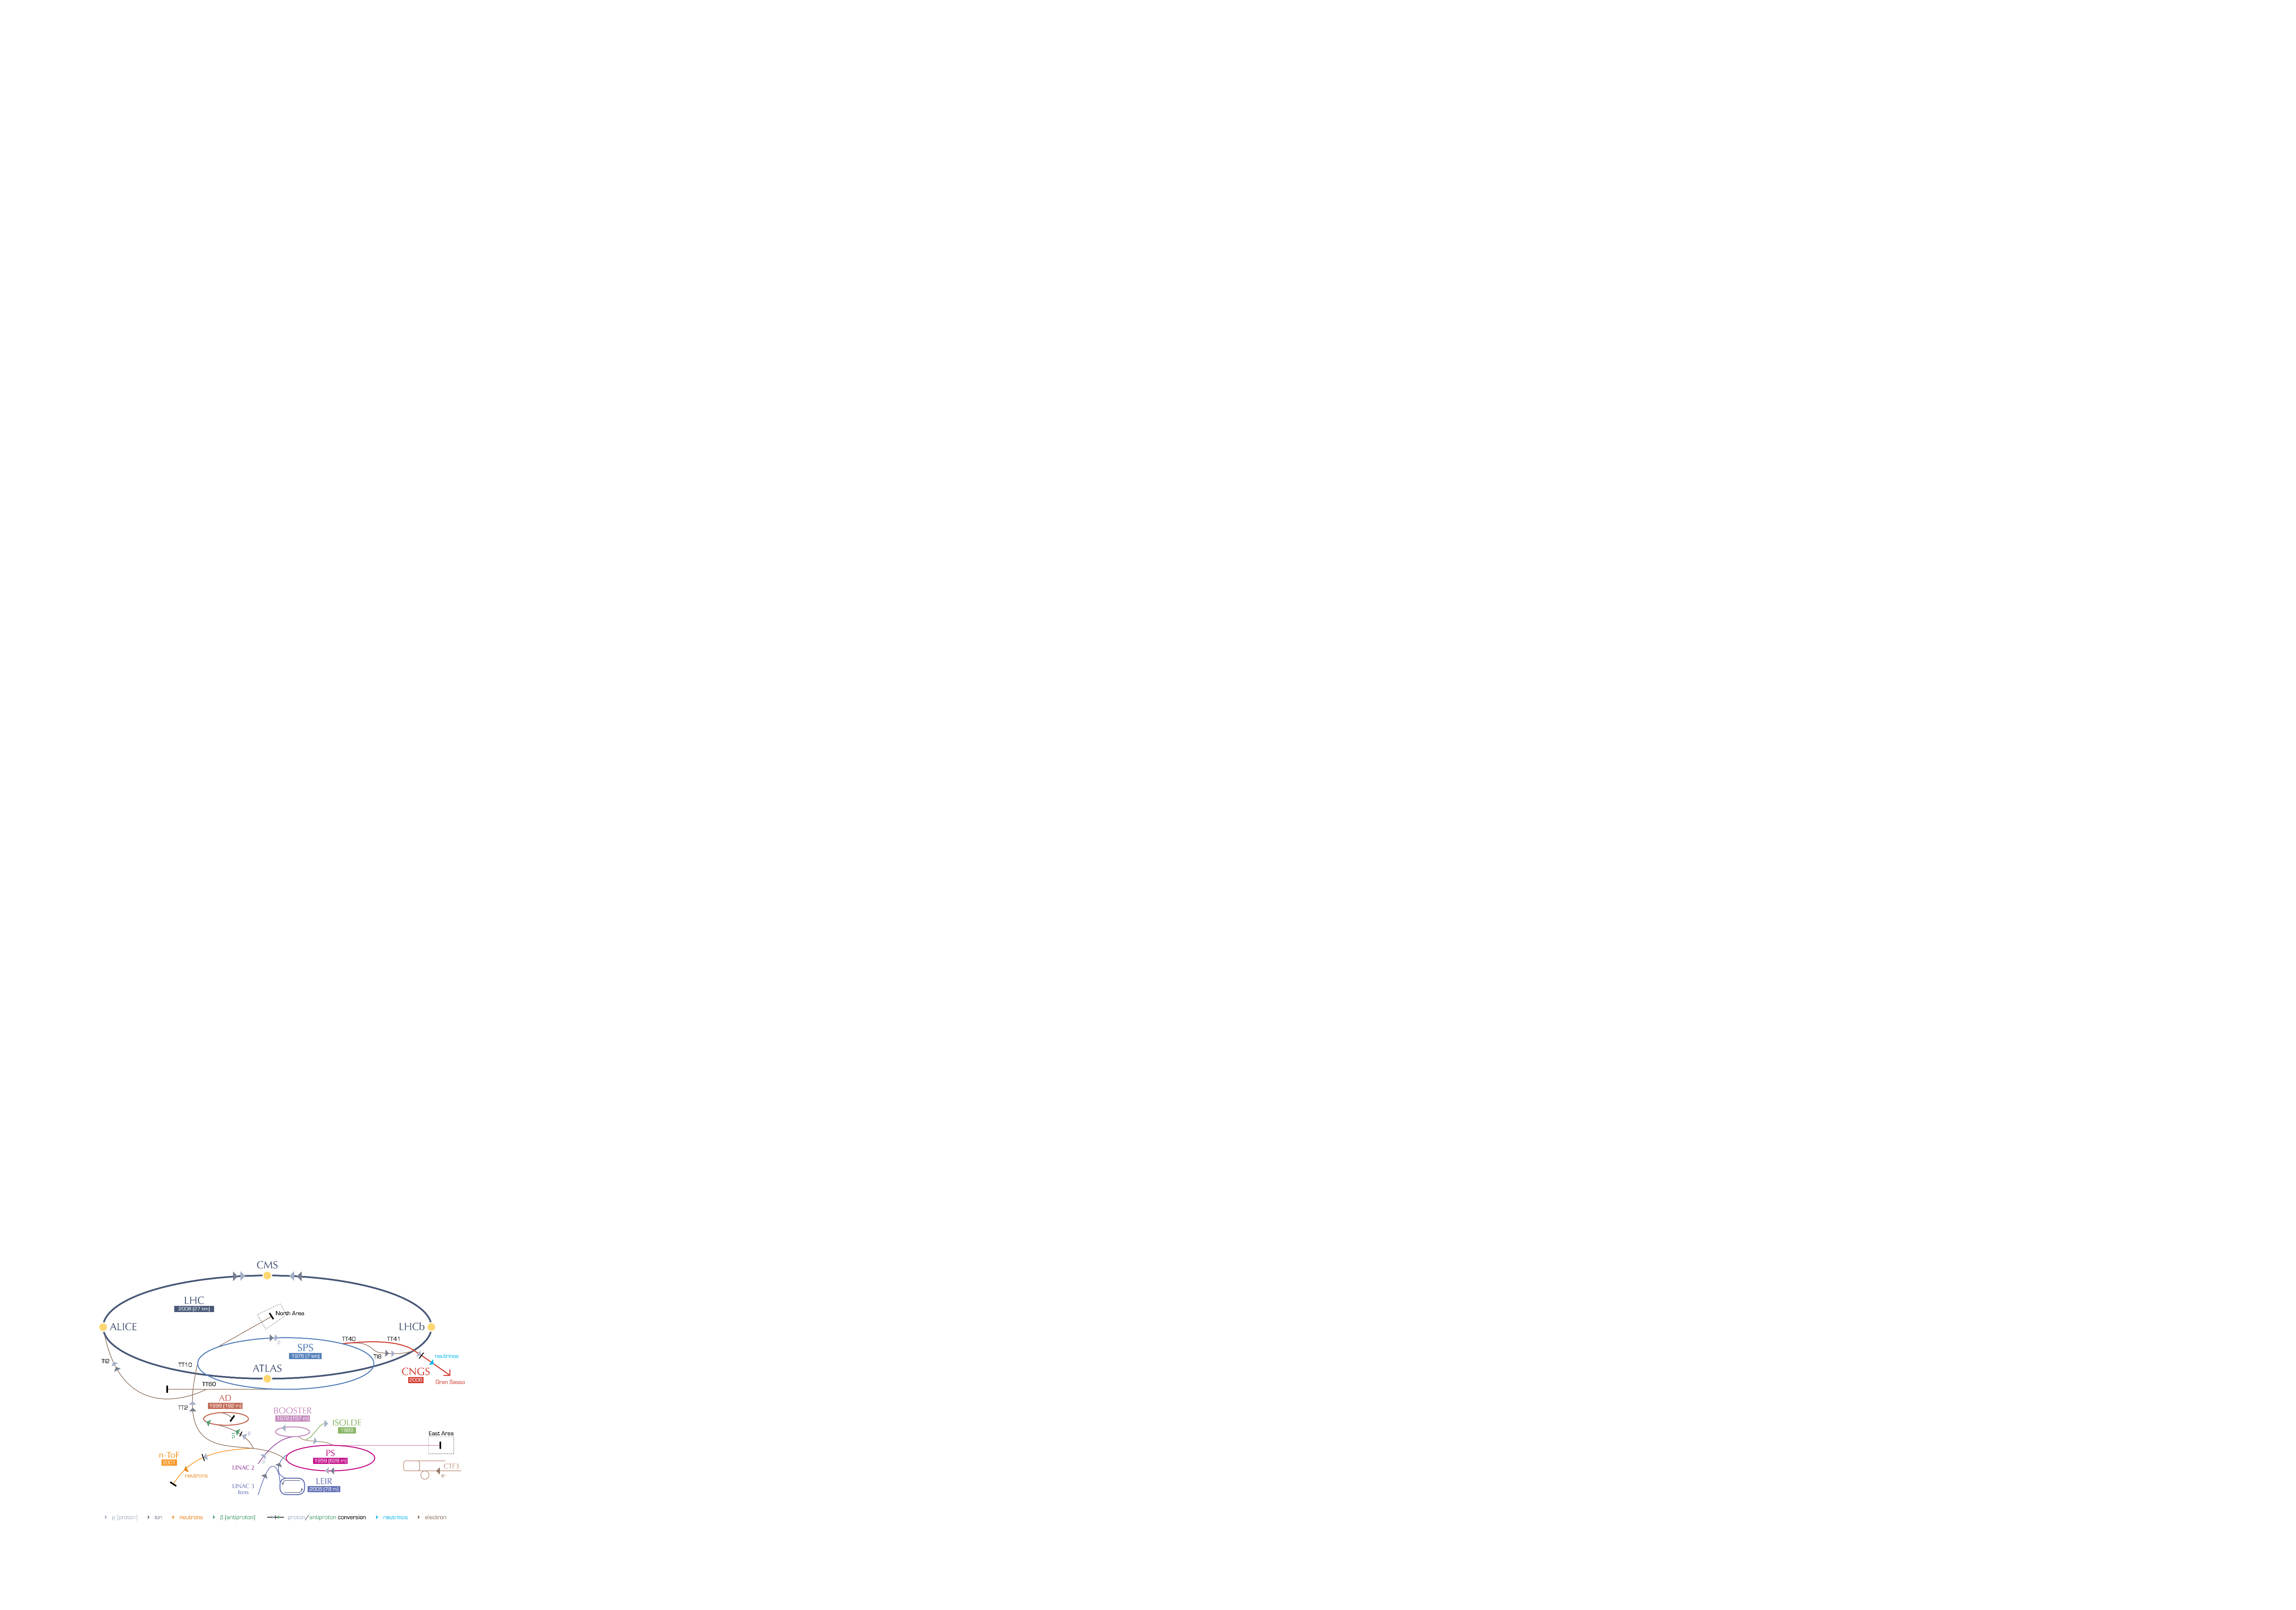
\includegraphics[width=1.0\textwidth]{figs/Detector/Acc_complex.pdf}
    \caption{The accelerator complex at \cern taken from Ref...}
    \label{fig:Dec_Acc_Complex}   
\end{figure}
%%%%%%%%%%%%%%%%%%%%%%%%%%%%%%%%%%%%%%%%%%%%%%%%%%%%%%%%%%



{\color{Red}
\begin{itemize}
\item Brief overview of the life of a proton from source to \lhc
\end{itemize}
}

\subsection{The \lhcb collaboration} 
{\color{Red}
\begin{itemize}
\item People and counties 
\item physics aims?
\end{itemize}
}
\subsection{Beam conditions at \lhcb}
{\color{Red}
\begin{itemize}
\item \lhc optics
\item crossing angle
\item Luminosity levelling
\end{itemize}
}


\section{The \lhcb detector}

This section provides an overview of the experimental apparatus used to obtain the data analysed in this thesis.
The \lhcb detector is comprised of distinct sub-detectors, each with a dedicated purpose. These help to characterise the sub-atomic particles created in the proton-proton collisions, and enable measurements of their kinematics, trajectories and species.
This overview includes a description of the sub-detector's construction, components and performance. 

The \lhcb detector is found at Point 8 of the \lhc ring, a cavern originally built for the {\color{Red}\delphi} detector during the \lep era. A schematic representing the key components of the \lhcb detector is shown in Fig.~\ref{fig:Dec_lhcb_Schematic}. This figure displays the axes convention adopted by \lhcb, and used henceforth. The horizontal axis is labelled the $z$-axis and is parallel to the direction of the beams. The figure's vertical axis is the $y$-axis, increasing as one moves from the cavern up to ground level. The $x$-axis is in the dimension perpendicular to the plane of the figure. The $x$-axis increases as one moves towards the centre of the \lhc ring. The counter-rotating beams of protons are collided at the far left of this figure, at the origins of the $y$- and $z$-axes.   

%%%%%%%%%%%%%%%%%%%%%%%%%%%%%%%%%%%%%%%%%%%%%%%%%%%%%%%%%%
\begin{figure}[!h]
    \centering
    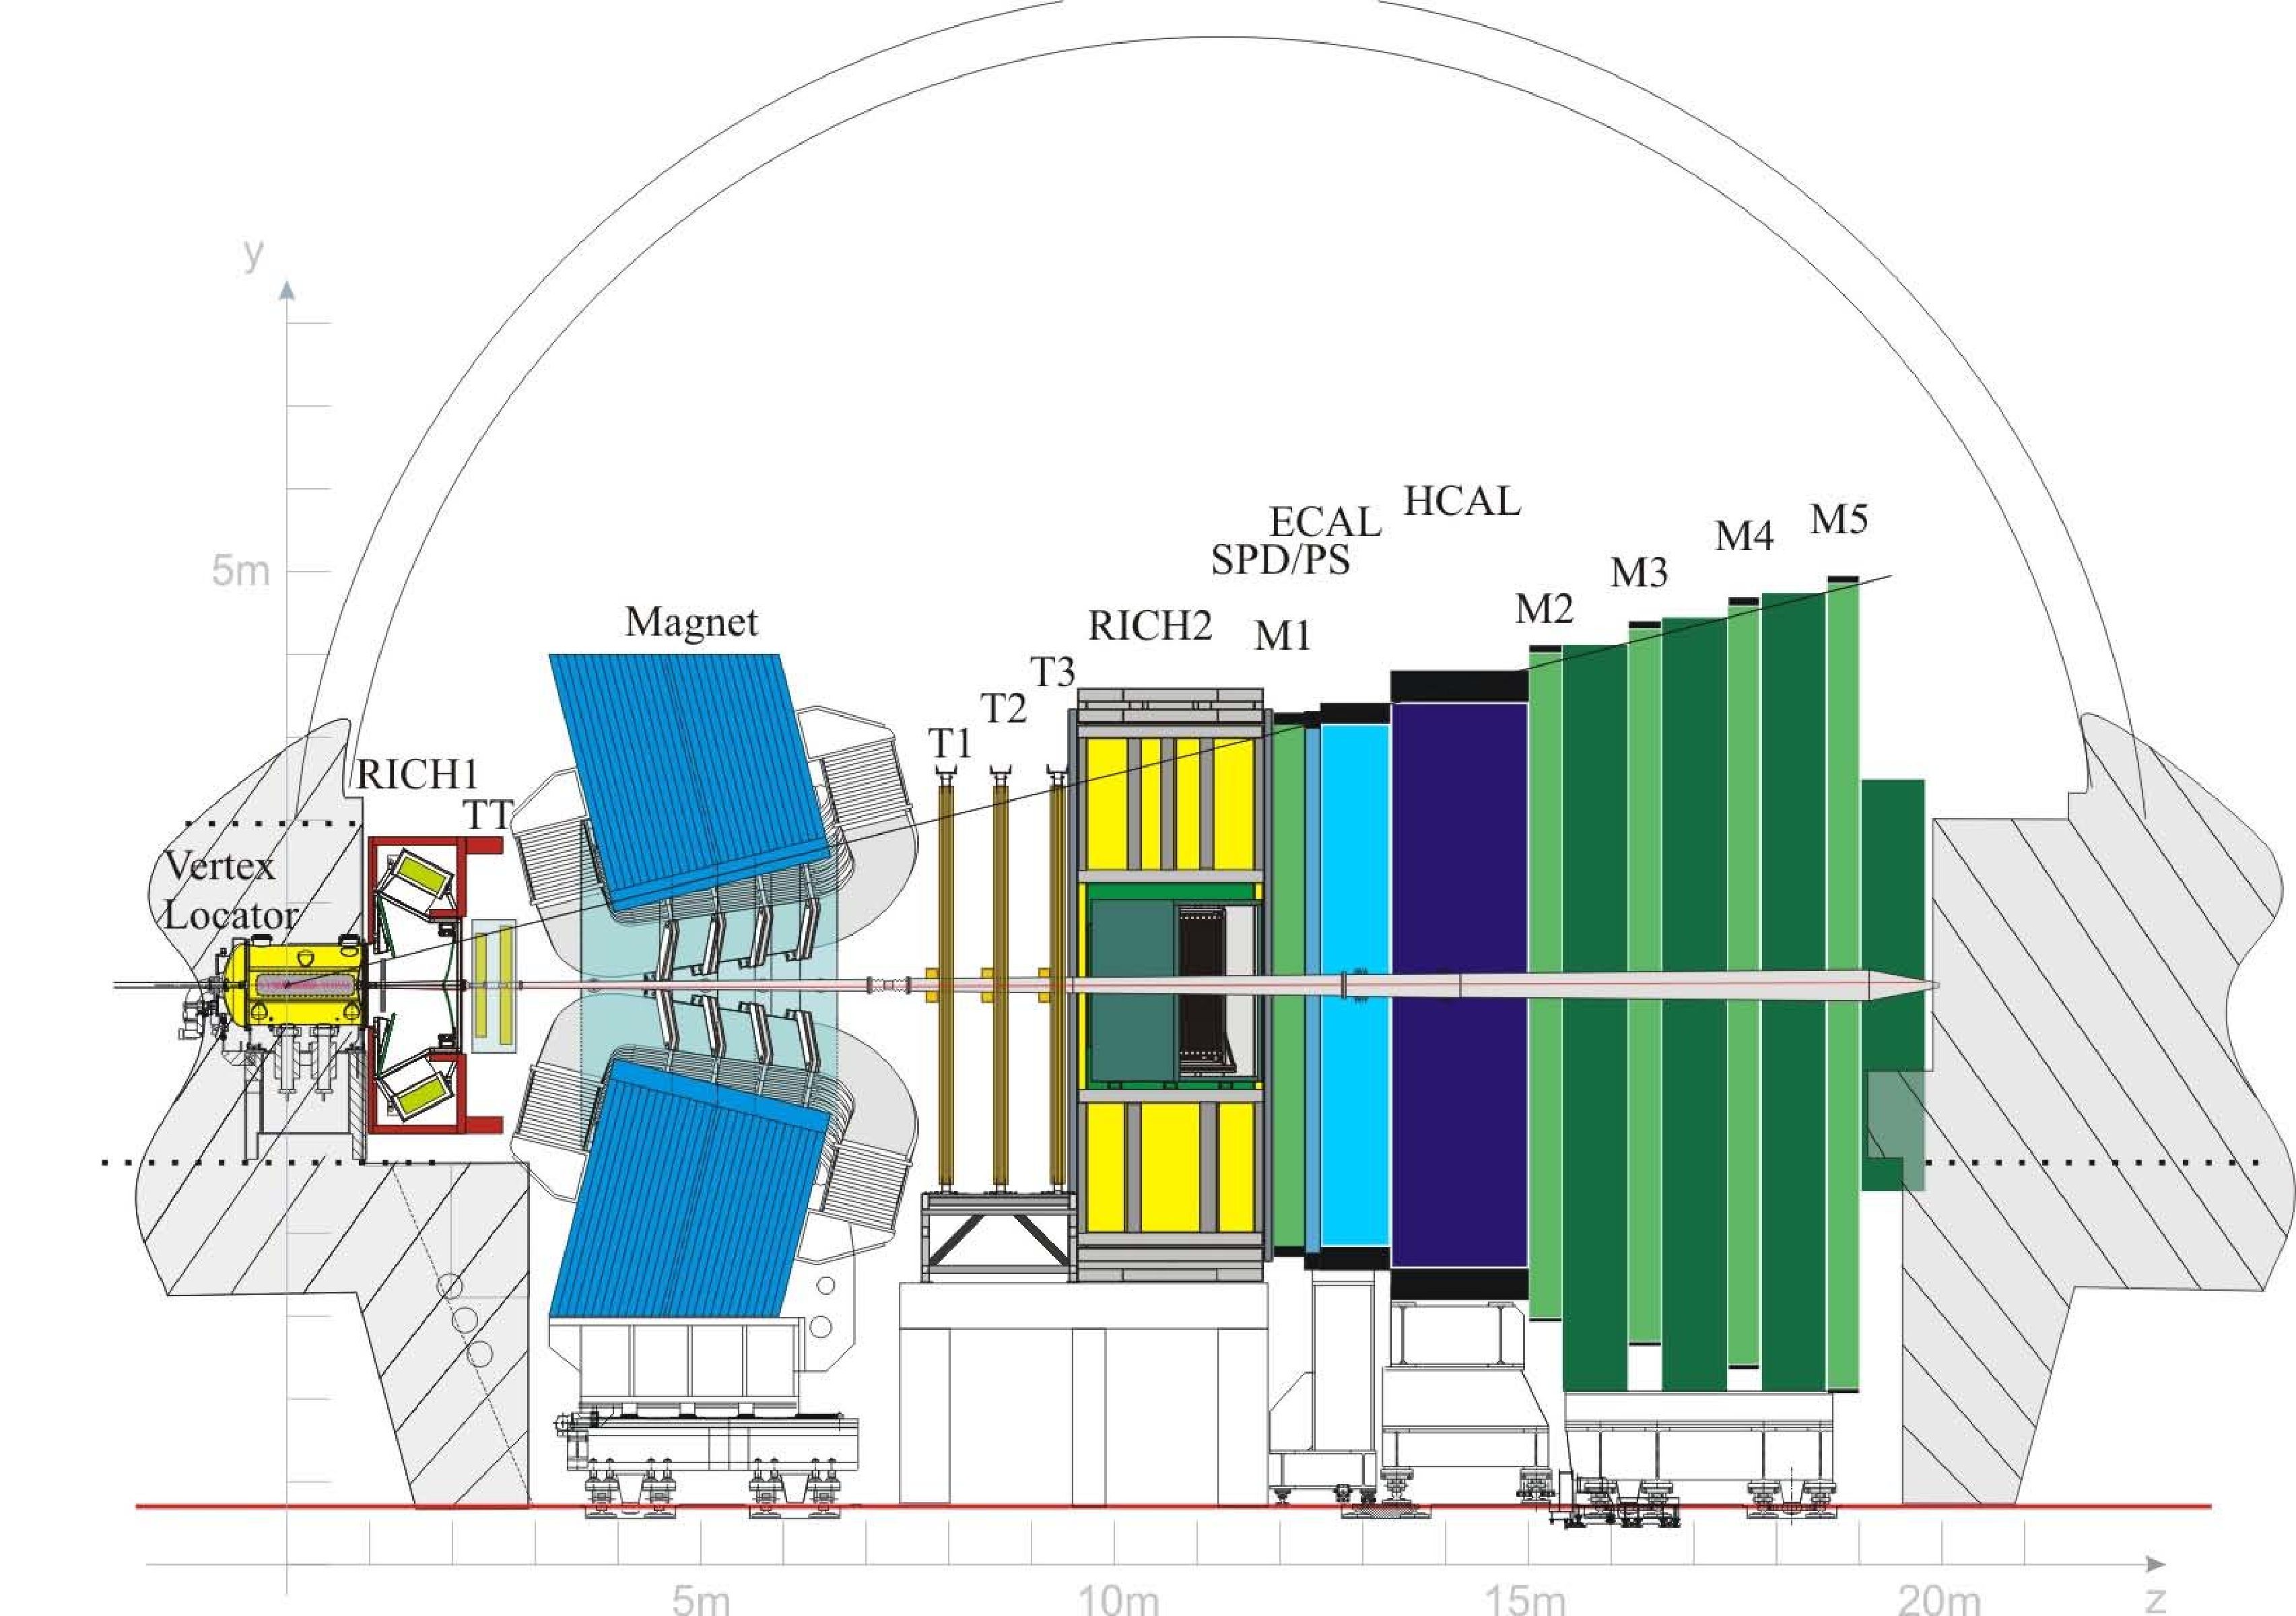
\includegraphics[width=0.8\textwidth]{figs/Detector/LHCb_Detector_Schematic.pdf}
    \caption{Schematic of the \lhcb detector from Ref.~\cite{Alves:2008zz}.}
    \label{fig:Dec_lhcb_Schematic}   
\end{figure}
%%%%%%%%%%%%%%%%%%%%%%%%%%%%%%%%%%%%%%%%%%%%%%%%%%%%%%%%%%



Running along the centre of the detector is the \lhcb beampipe. The primary role is to separate the inner vacuum chamber from the rest of the cavern, allowing the beams to proceed unimpeded by the air. The majority of the beampipe is made of beryllium, with smaller sections made out of aluminium alloys or stainless steel. Although beryllium is a highly toxic and fragile material it has a long radiation length, allowing the incident particles to traverse the pipe walls with minimal interactions.  


{\color{Red}
\begin{itemize}
\item Cavern
\item Beam pipe
\item Define axes 
\end{itemize}
}

{\color{Green}
\begin{itemize}
\item Distribution of bb pairs
\end{itemize}
}

\subsection{Magnet}

The \lhcb detector contains a warm dipole magnet that bends the trajectories of charges particles, allowing measurements of the particles' momentum. The magnet has two saddle-shaped coils inside a square yoke that generate an integrated magnetic field of 4 Tm.  
The magnetic field is aligned along the $y$-axis, bending the charged particles in the horizontal plane. The polarity of the magnetic is routinely switched during data taking. This helps to understand and cancel systematic effects that may affect measurements of \CP asymmetries. The two magnet polarities are referred to \emph{MagDown} and \emph{MagUp}, corresponding to a field in the negative and positive $y$-axis direction respectively.   

A schematic of the magnet is shown in Fig.~\ref{fig:Dec_magnet}, along with the strength of the magnetic field as a function of the $z$-axis position. Both magnet polarities are represented in this figure. 

{\color{Red}
\begin{itemize}
\item Magnet: purpose and design 
\end{itemize}
}


%%%%%%%%%%%%%%%%%%%%%%%%%%%%%%%%%%%%%%%%%%%%%%%%%%%%%%%%%%
\begin{figure}[!h]
    \centering
    \begin{subfigure}[t]{0.4\textwidth}
        \centering
        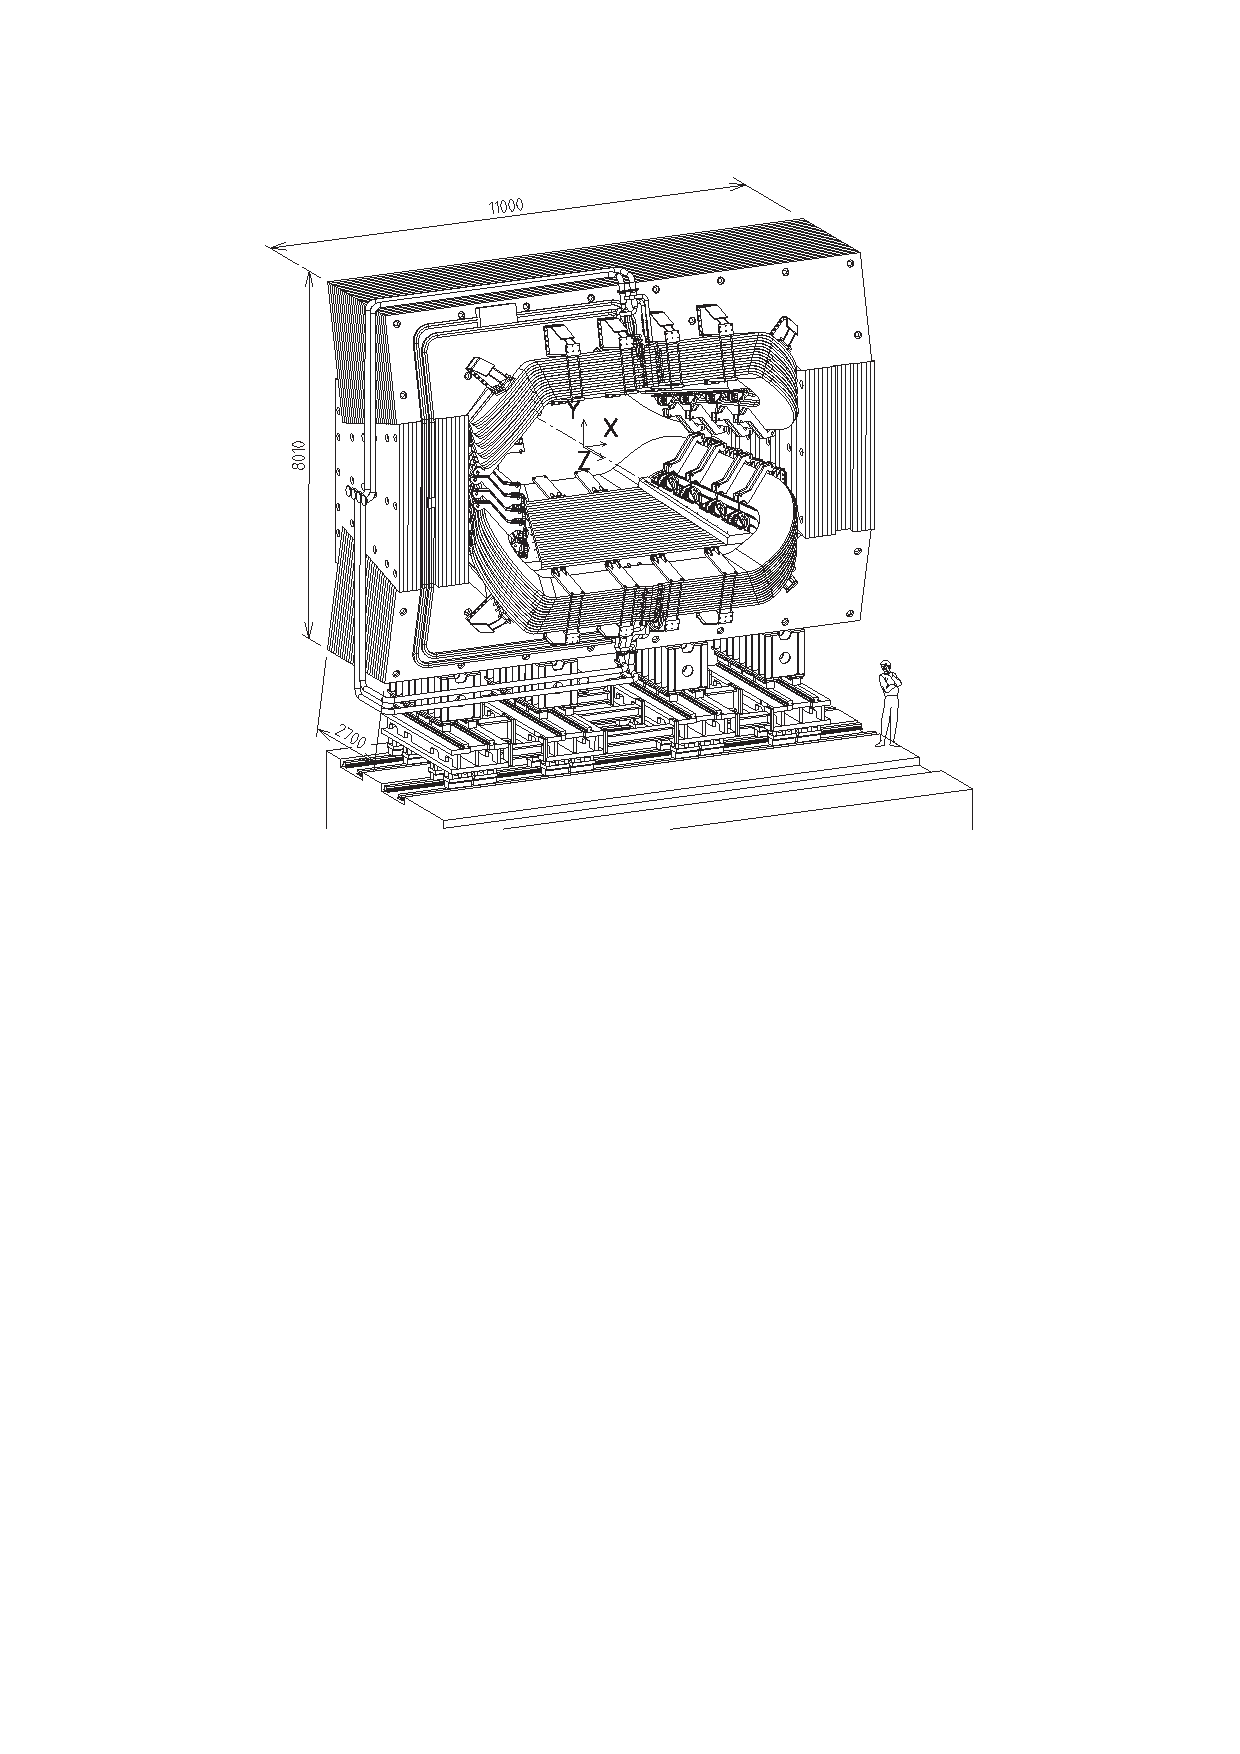
\includegraphics[width=1.0\textwidth]{figs/Detector/magnet_schematic.pdf}
    \end{subfigure}
    \begin{subfigure}[t]{0.4\textwidth}
        \centering
        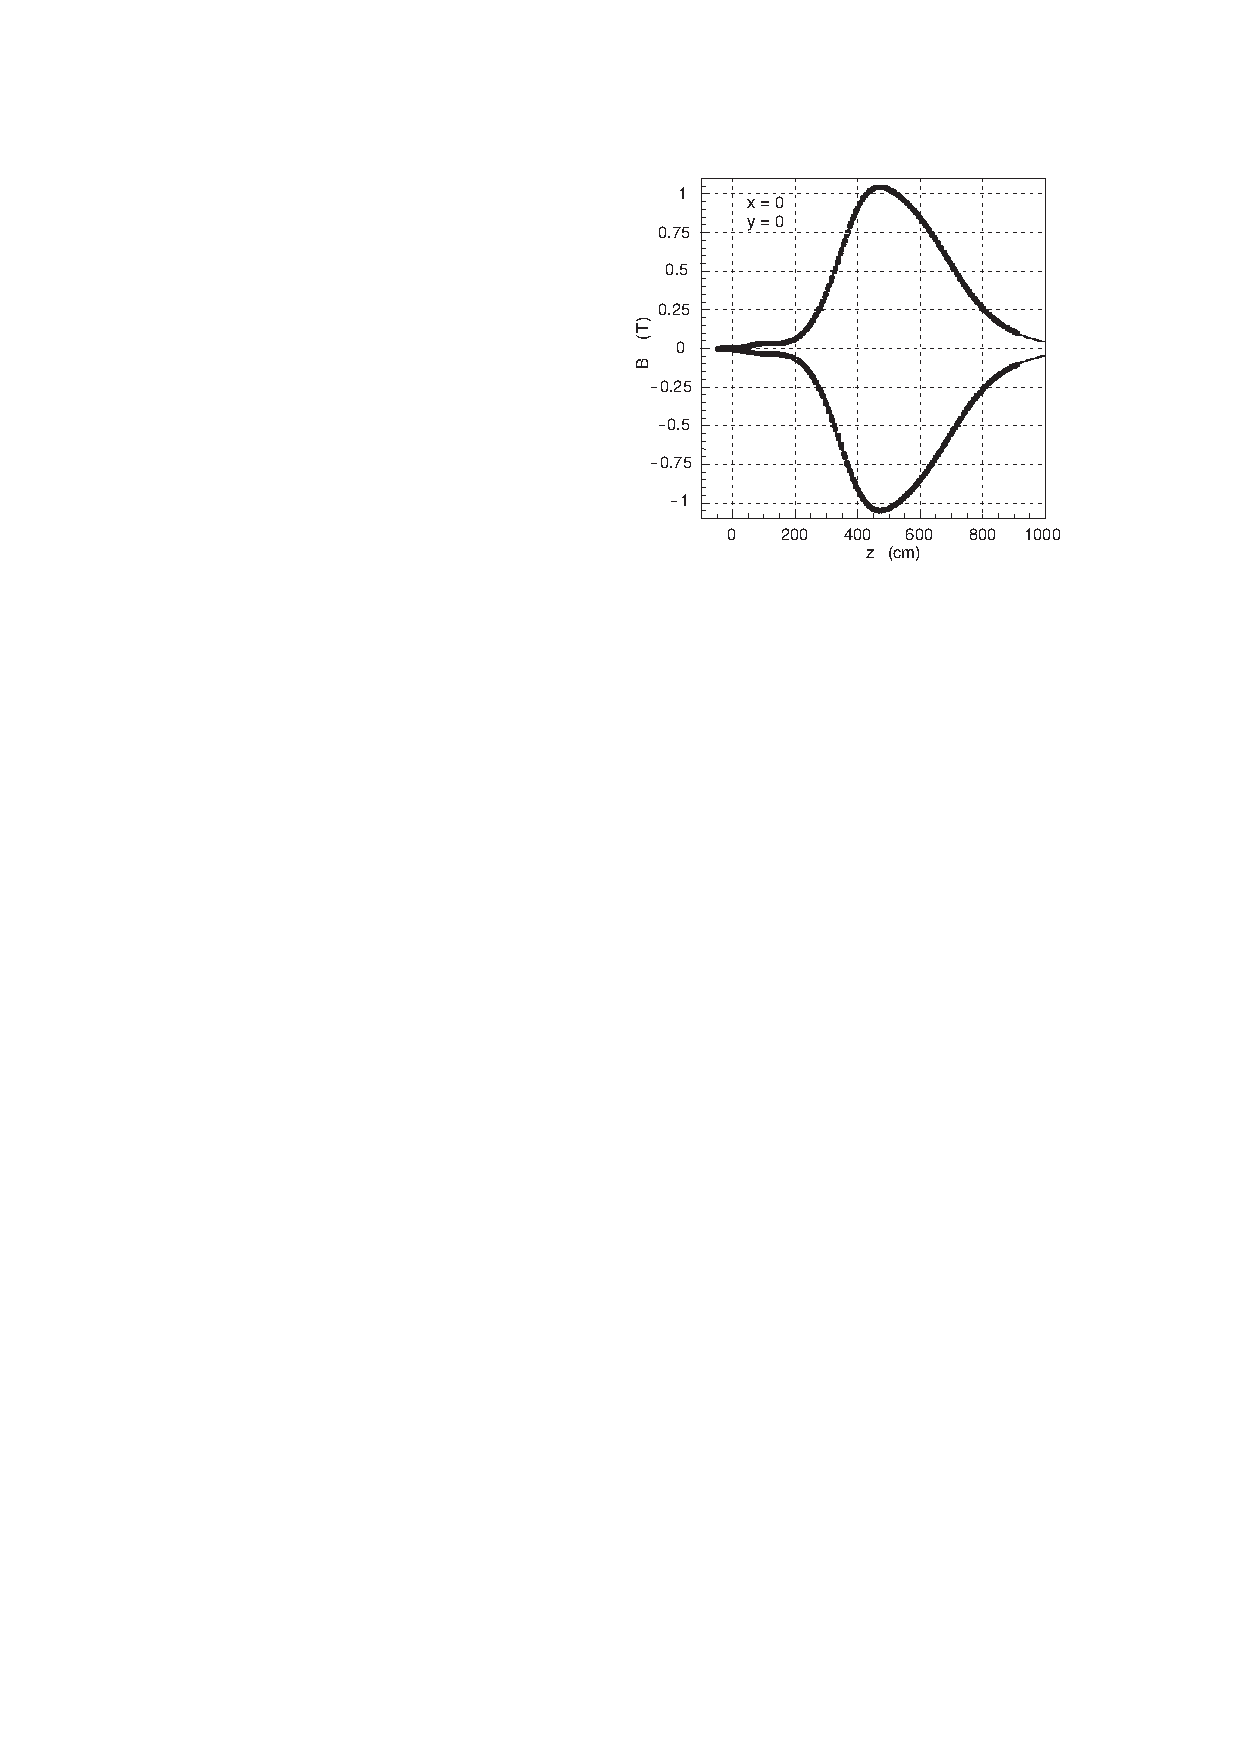
\includegraphics[width=1.0\textwidth]{figs/Detector/magnet_B_field.pdf}
    \end{subfigure}
    \caption{Schematic of the \lhcb warm dipole magnet (left) and the magnetic field strength along the $z$-axis (right) from Ref.~\cite{Alves:2008zz}.}
    \label{fig:Dec_magnet}   
\end{figure}
%%%%%%%%%%%%%%%%%%%%%%%%%%%%%%%%%%%%%%%%%%%%%%%%%%%%%%%%%%


\subsection{Vertex Locator}

The first sub-detector to make measurements of the particles produced in proton-proton collisions is the Vertex Locator (\velo) encompassing the collision region. This sub-detector make precise measurements of the track positions of charged particles as they emanate out of the collisions. A high level of precision is required to identify the secondary vertices characteristic of \bquark- and \cquark-hadron decays. These secondary vertices are typically displaced from the interaction position as a result of the long lifetimes associated to these heavy-flavour hadrons. This is achieved by measuring the track coordinates using silicon sensors 


%%%%%%%%%%%%%%%%%%%%%%%%%%%%%%%%%%%%%%%%%%%%%%%%%%%%%%%%%%
\begin{figure}[!h]
    \centering
    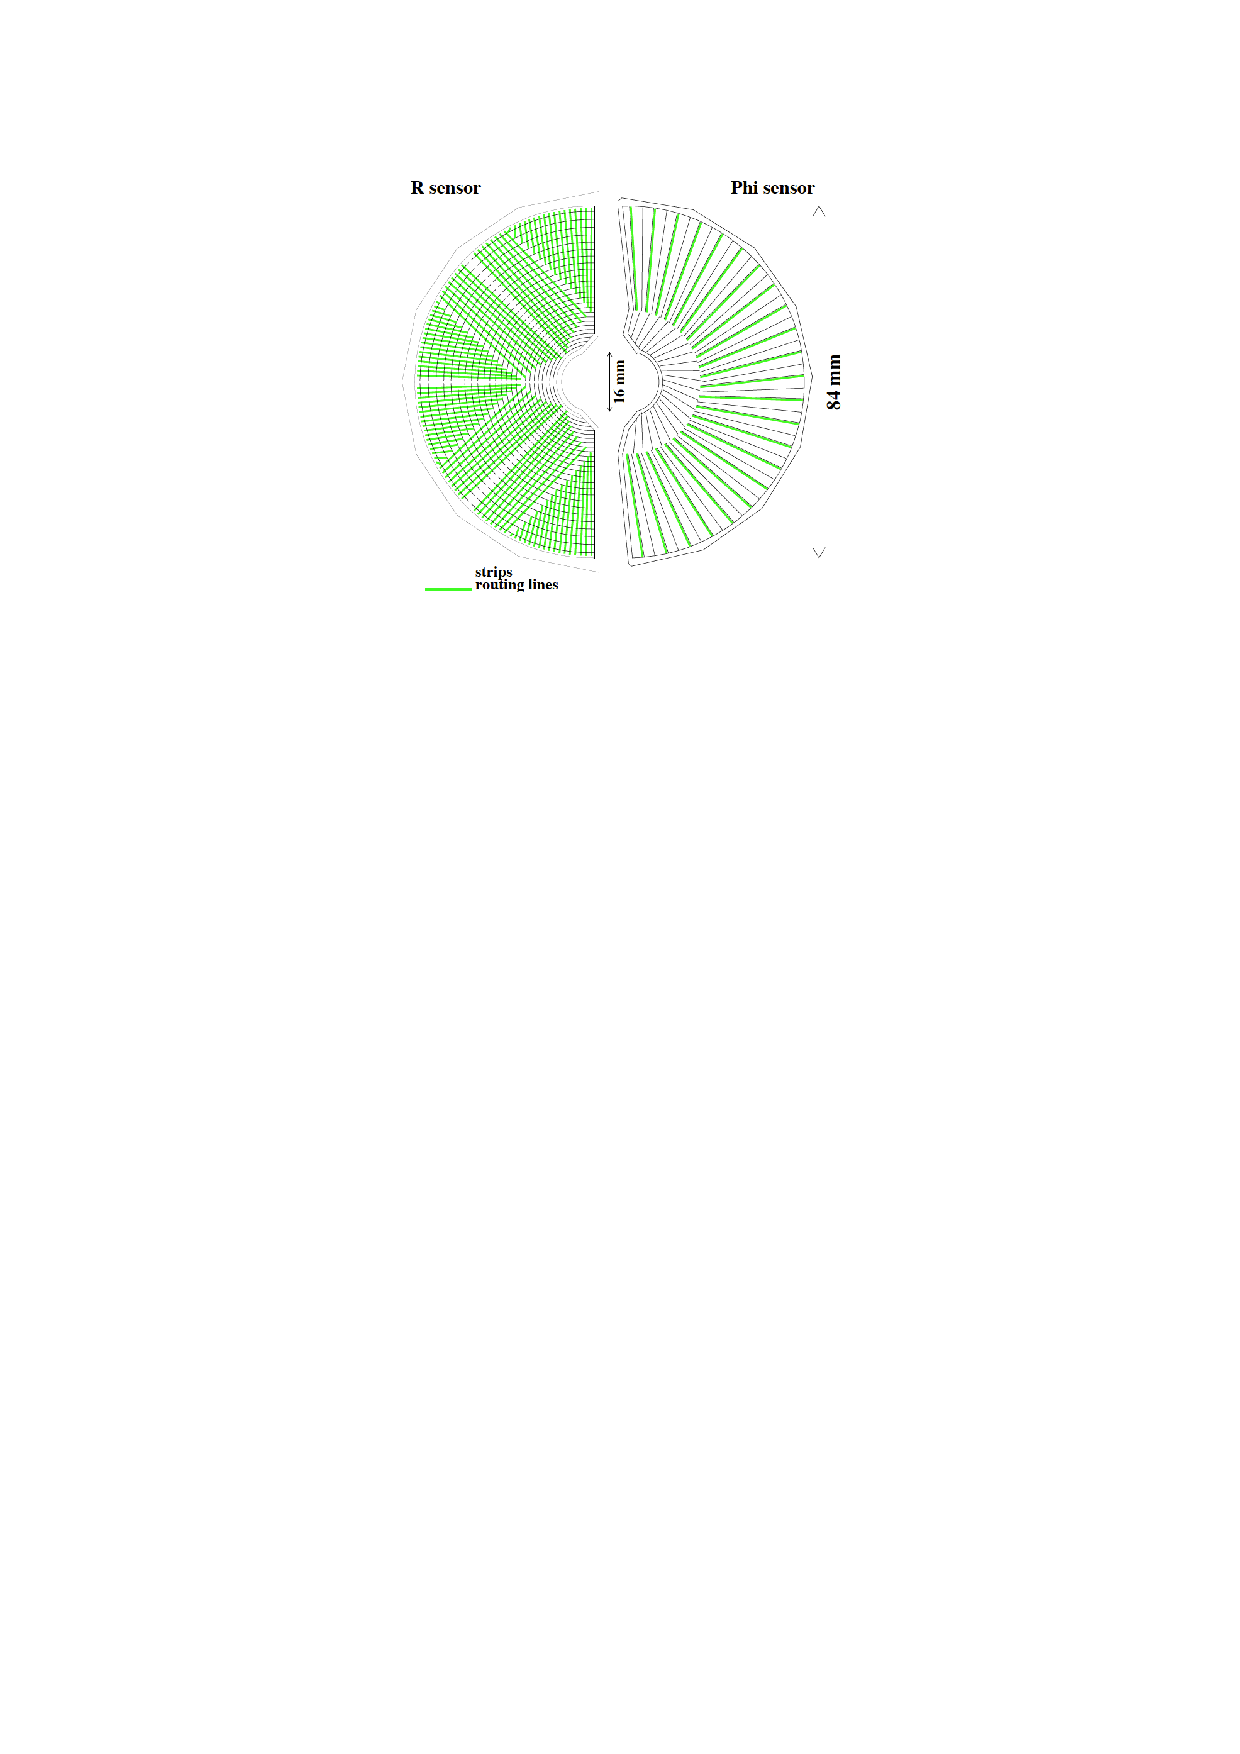
\includegraphics[width=0.4\textwidth]{figs/Detector/velo_r_phi_sensor.pdf}
    \caption{Schematic of an $r$- and $\phi$-sensor in the \velo sub-detector from Ref.~\cite{LHCb-DP-2014-001}.}
    \label{fig:Dec_velo_sensor_Schematic}   
\end{figure}
%%%%%%%%%%%%%%%%%%%%%%%%%%%%%%%%%%%%%%%%%%%%%%%%%%%%%%%%%%


{\color{Red}
\begin{itemize}
\item two halves, and moving
\item RF foil?
\item 
\item velo read out chain
\item performance in run1 and run2: track finding efficiency 
\end{itemize}
}




\subsection{Silicon Tracker}
\subsection{Outer Tracker}
\subsection{Ring imaging Cherenkov detectors}
\subsubsection{\richone}
\subsubsection{\richtwo}
\subsection{Calorimeters}
\subsubsection{Pre-shower detector}
\subsubsection{Electronic Calorimeter}
\subsubsection{Hadron calorimeter}
\subsection{Muon system}
\subsection{Trigger}
\subsubsection{\lone}
\subsubsection{\hltone}
\subsubsection{\hlttwo}


\section{VELO resolution and luminosity determination}